\documentclass{beamer}

% NOTE: reference
% https://arxiv.org/pdf/1604.05488.pdf



\mode<presentation> {\usetheme{Madrid}}

\usepackage{graphicx}
\usepackage[utf8]{inputenc}
\usepackage{amsmath, amsthm, amssymb, mathtools}
\usepackage{hyperref}
\usepackage{flexisym}
\graphicspath{{./img/}}

\title[TeV Astrophysics]{Astronomical facilities and instrumentation in TeV}

\author{Wei-Chih Huang}
\institute[NTHU]{
National Tsing Hua University \\
\medskip
}
\date{April 23, 2019}


\begin{document}

\begin{frame}
	\titlepage % Print the title page as the first slide
\end{frame}

\begin{frame}{Overview}
	\tableofcontents
\end{frame}




\section{Introduction to Tev $\gamma$ ray}
%%%%%%%%%%%%%%%%%%%%%%%%%%%%%%%%%%%%%%%%%%%%%%
\begin{frame}{Introduction to Tev $\gamma$ ray}
	\begin{itemize}
		\item $\gamma$ ray production mechanisms
		\item Astrophysical sources of high-energy $\gamma$ rays
		\item Detection method
		\item Cherenkov radiation
	\end{itemize}
\end{frame}



\subsection{$\gamma$ ray production mechanisms}
\begin{frame}{$\gamma$ ray production mechanisms}
	There are several ways to generate cosmic gamma rays:
	\begin{enumerate}
		\item $p_1 + p_2 \rightarrow \gamma + q_1 + ...$
		\item $p^+ + p^- \rightarrow \gamma + \gamma$
		\item $p_0 \rightarrow \gamma + q_1 + ...$
		\item $p \xrightarrow{\text{accelerate}} \gamma + p$
	\end{enumerate}

	Examples:
	\begin{enumerate}
		\item $p_i = proton, nucleus, q = pion \text{ (which decay into a pair of gamma rays)}$
		\item $p^+ = position, p^- = electron$
		\item $p_0 = \text{some heavy nuclei}$
		\item synchrotron radiation $P = \frac{2Ke^2 \gamma^4 v^4}{3c^3r^2} $
	\end{enumerate}
	\setlength{\fboxrule}{0.1pt}{hello}
	\href{https://imagine.gsfc.nasa.gov/science/toolbox/gamma_generation.html}{some animation}
\end{frame}



\subsection{Astrophysical sources of high-energy $\gamma$ rays}
\begin{frame}{Astrophysical sources of high-energy $\gamma$ rays}
	\begin{enumerate}
		\item pulsars
		\item blazars
		\item AGN
		\item pulsar wind nebula
		\item supernova remnant
		\item some particular binary system
		\item the centre of Galaxy
	\end{enumerate}
\end{frame}



\subsection{Detection method}
\begin{frame}{Ground-based detector}
	challenges:
	\begin{itemize}
		\item High-energy $\gamma$ ray cannot be focused.
		\item Above 100 MeV, $\gamma$ rays can only be detected by their conversion into $e^+ + e^-$ pairs in matter
		\item electromagnetic cascade
	\end{itemize}

	solutions:
	\begin{itemize}
		\item more sensitive detector
		\item higher altitude experiment
	\end{itemize}
\end{frame}


\begin{frame}{Space-based detector}

\end{frame}



\subsection{Cherenkov radiation}
\begin{frame}{Cherenkov radiation}
	\begin{figure}[h]
		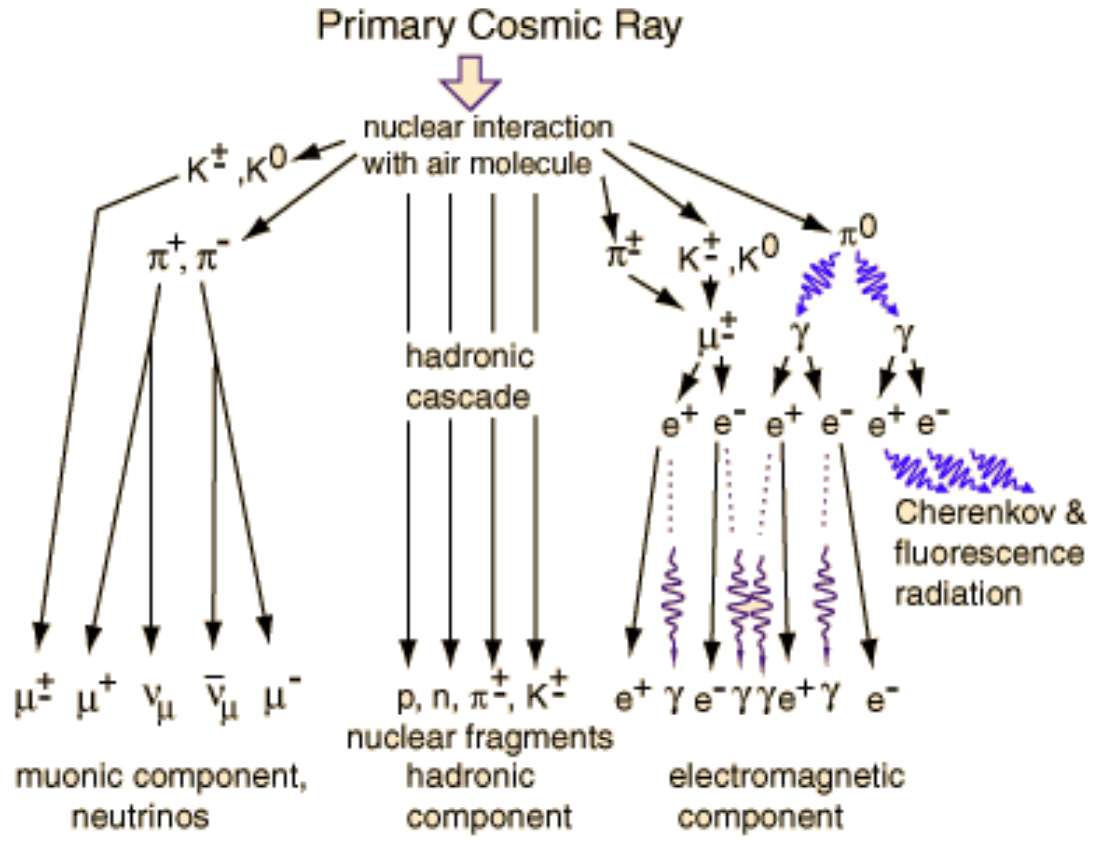
\includegraphics[width=280px]{cara.png}
	\end{figure}
\end{frame}

\begin{frame}{Cherenkov radiation}
	\begin{figure}[h]
		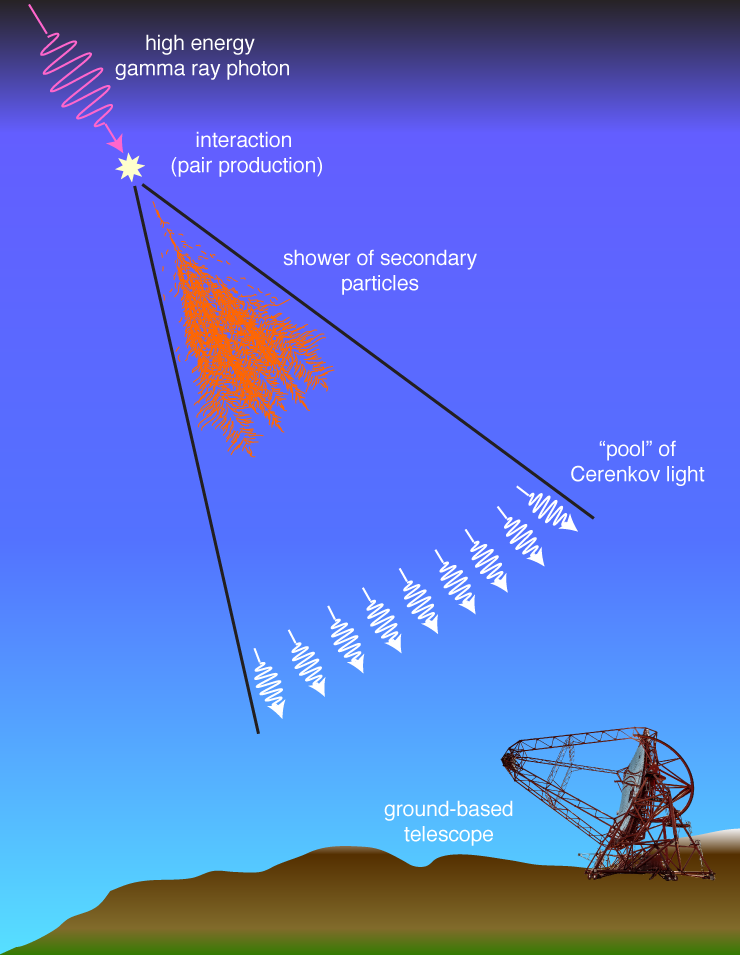
\includegraphics[width=170px]{atmosphere_cerenkov.png}
	\end{figure}
\end{frame}


\section{Detectors}
%%%%%%%%%%%%%%%%%%%%%%%%%%%%%%%%%%%%%%%%%%%%%%
\begin{frame}{Detectors}
	\begin{itemize}
		\item OSO-3 satellite detector
		\item ICAT

	\end{itemize}
\end{frame}

\subsection{OSO-3 satellite}
\begin{frame}{OSO-3 satellite}
	OSO 3 (Orbiting Solar Observatory 3)

	\begin{enumerate}
		\item Mar. 8, 1967: launched on
		\item Jun. 28, 1968: tape recorder failed
		\item Nov. 10, 1969: last data were received
		\item Apr. 4, 1982: burned up
	\end{enumerate}
	Result:
	\newline
	The MIT gamma-ray instrument obtained the first identification of high-energy cosmic gamma rays emanating from both galactic and extra-galactic sources
\end{frame}



\subsection{ICAT}
\begin{frame}{ICAT Properties}
	Properties:
	\begin{enumerate}
		\item 50 GeV ~ 50 TeV in photon energy range
		\item ground-based detector
		\item Wider energy regime than space-based instruments
		\item largest telescope at the highest altitude
		\item work by detecting Cherenkov radiation produced by high energy charged particles
	\end{enumerate}
\end{frame}



\begin{frame}{ICAT components}
	Imaging Atmospheric (or Air) Cherenkov Telescope or Technique
	\newline
	\newline
	Four operating IACT systems:
	\begin{enumerate}
		\item High Energy Stereoscopic System (H.E.S.S.)
		\item Major Atmospheric Gamma Imaging Cherenkov Telescopes (MAGIC)
		\item First G-APD Cherenkov Telescope (FACT)
		\item Very Energetic Radiation Imaging Telescope Array System (VERITAS)
	\end{enumerate}
\end{frame}

\begin{frame}{ICAT components}
	\begin{figure}[h]
		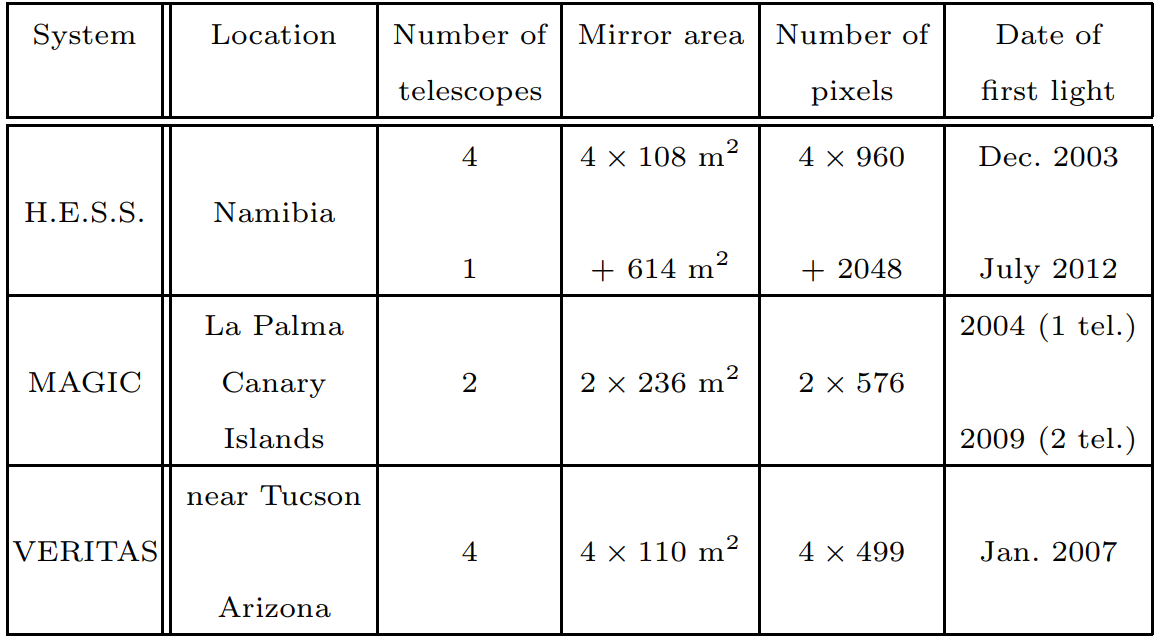
\includegraphics[width=280px]{ICATsystems.png}
	\end{figure}
\end{frame}


\begin{frame}{ICAT components}
	\begin{figure}[h]
		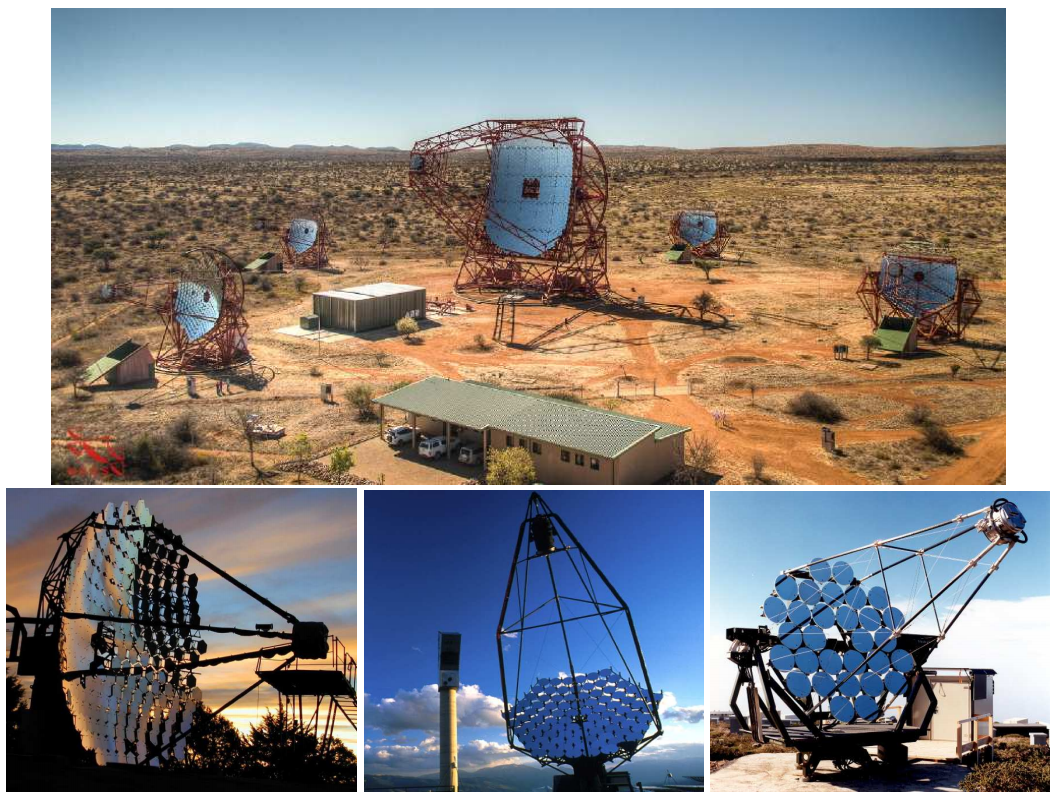
\includegraphics[width=200px]{dishes.png}
		\caption{Illustration of the combination in H.E.S.S. (upper panel) of large dishes as in Whipple (lower left), fast and fine grained cameras as in CAT (lower centre) and stereoscopic observation as in HEGRA (lower right)].}
	\end{figure}
\end{frame}


\end{document}